%%%%%%%%%%%%%%%%%%%%%%%%%%%%%%%%%%%%%%%%%
% University/School Laboratory Report
% LaTeX Template
% Version 3.1 (25/3/14)
%
% This template has been downloaded from:
% http://www.LaTeXTemplates.com
%
% Original author:
% Linux and Unix Users Group at Virginia Tech Wiki 
% (https://vtluug.org/wiki/Example_LaTeX_chem_lab_report)
%
% License:
% CC BY-NC-SA 3.0 (http://creativecommons.org/licenses/by-nc-sa/3.0/)
%
%%%%%%%%%%%%%%%%%%%%%%%%%%%%%%%%%%%%%%%%%

\documentclass[paper=letter, fontsize=11pt]{article}

% packages
\usepackage{fixltx2e}
\usepackage[pdftex]{graphicx}
\usepackage{color, wrapfig}
\usepackage{amsmath}  % required for some math elements 
\usepackage{fancyvrb, listings}  % for code verbatim and console outputs
\usepackage[margin=1in]{geometry}

\definecolor{dkgreen}{rgb}{0,0.6,0}
\definecolor{gray}{rgb}{0.5,0.5,0.5}
\definecolor{mauve}{rgb}{0.58,0,0.82}
\definecolor{black}{rgb}{0,0,0}

\lstset{frame=tb,
    language=R,
    aboveskip=3mm,
    belowskip=3mm,
    showstringspaces=false,
    columns=flexible,
    basicstyle={\small\ttfamily},
    numbers=none,
    numberstyle=\tiny\color{gray},
    keywordstyle=\color{blue},
    commentstyle=\color{dkgreen},
    stringstyle=\color{mauve},
    breaklines=true,
    breakatwhitespace=true,
    tabsize=4,
    escapechar={\?}
}

\setlength\parindent{0pt} % removes all indentation from paragraphs

% redefine \VerbatimInput
\RecustomVerbatimCommand{\VerbatimInput}{VerbatimInput}{
    fontsize=\footnotesize,
    frame=lines,  % top and bottom rule only
    framesep=2em,  % separation between frame and text
    rulecolor=\color{black},
    label=\fbox{\color{black}main.R},
    labelposition=topline,
}

%----------------------------------------------------------------------------------------
%	DOCUMENT INFORMATION
%----------------------------------------------------------------------------------------

\title{Project 2 \\ STAT 355}  % Title
\author{Sabbir \textsc{Ahmed}}  % Author name
\date{\today}  % Date for the report

\begin{document}

    \maketitle % Insert the title, author and date

    % ------------------------------ Part 1 ------------------------------
    \section{Part 1}
        1000 random samples of size 40 were generated from normal distribution with mean $\mu$ = 3 and standard deviation $\sigma$ = 2.

\begin{lstlisting}
    # initialize parameters for normal distribution
    N <- 40  # size
    mu <- 3  # mean
    sigma <- 2  # standard deviation

    sampMeans <- randDist(N, mu, sigma, "normal", "part1.tex")
    plotHist(sampMeans, "hist1.png", 0.1)
\end{lstlisting}

        \section{Part 1}
    \subsection{Question}
    An oceanographer wants to test, on the basis of a random sample of size 35, whether the average depth of the ocean in a certain area is 72.4 fathoms. At the 0.05 level of significance, what will the oceanographer decide if she gets a sample mean of 73.2? Assume the population standard deviation is 2.1.

    \subsection{Answer}
    The null hypothesis, $H_{0}$, claims the mean depth of the ocean in a certain area is 72.4, while the alternative hypothesis, $H_{a}$, says otherwise.

        \[ H_{0}: \mu = 72.4 \ vs \ H_{a}: \mu \neq 72.4 \]

    Since the population mean and standard deviation are known with a sample size of $n > 30$, the Z-score was calculated as follows:

        \begin{equation*}
    Z=\frac{\overline{X}-\mu}{\sfrac{\sigma}{\sqrt{n}}}
    =\frac{73.2-72.4}{\sfrac{2.1}{\sqrt{35}}}=2.2537
    \end{equation*}\newline

    The following snippet was used to generate the Z-test and its probability:
\begin{lstlisting}
    X <- 73.2
    mu <- 72.4
    sigma <- 2.1
    n <- 35
    alpha <- 0.05

    dumpComputation(X=X, mu=mu, sigma=sigma, n=n, 
        alpha=alpha, distType="Z", twoSided=TRUE, "part1")
\end{lstlisting}

    The test statistic was computed to be:

    \begin{equation*}
        Z_{1-\sfrac{0.05}{2}}=Z_{0.975}= 1.96 < 2.2537
    \end{equation*}

    The p-value was computed with the following snippet:
\begin{lstlisting}
    pScore <- 2 * (1 - (pnorm(score)))
    # 0.0242
\end{lstlisting}

    Since $Z_{\sfrac{\alpha}{2}} < Z$ and the p-score was under 0.05, the null hypothesis is rejected.


        \subsection{Distribution}
            Distribution of the data was plotted with a histogram using ggplot2 in Figure \ref{fig:hist1}.
\begin{lstlisting}
    ggplot() + aes(sampMeans) + 
        geom_histogram(binwidth=0.1, color="black", fill="white") +
        labs(y="Count", x="Sample Means")
\end{lstlisting}

            \begin{figure}[!h]
                \begin{center}
                    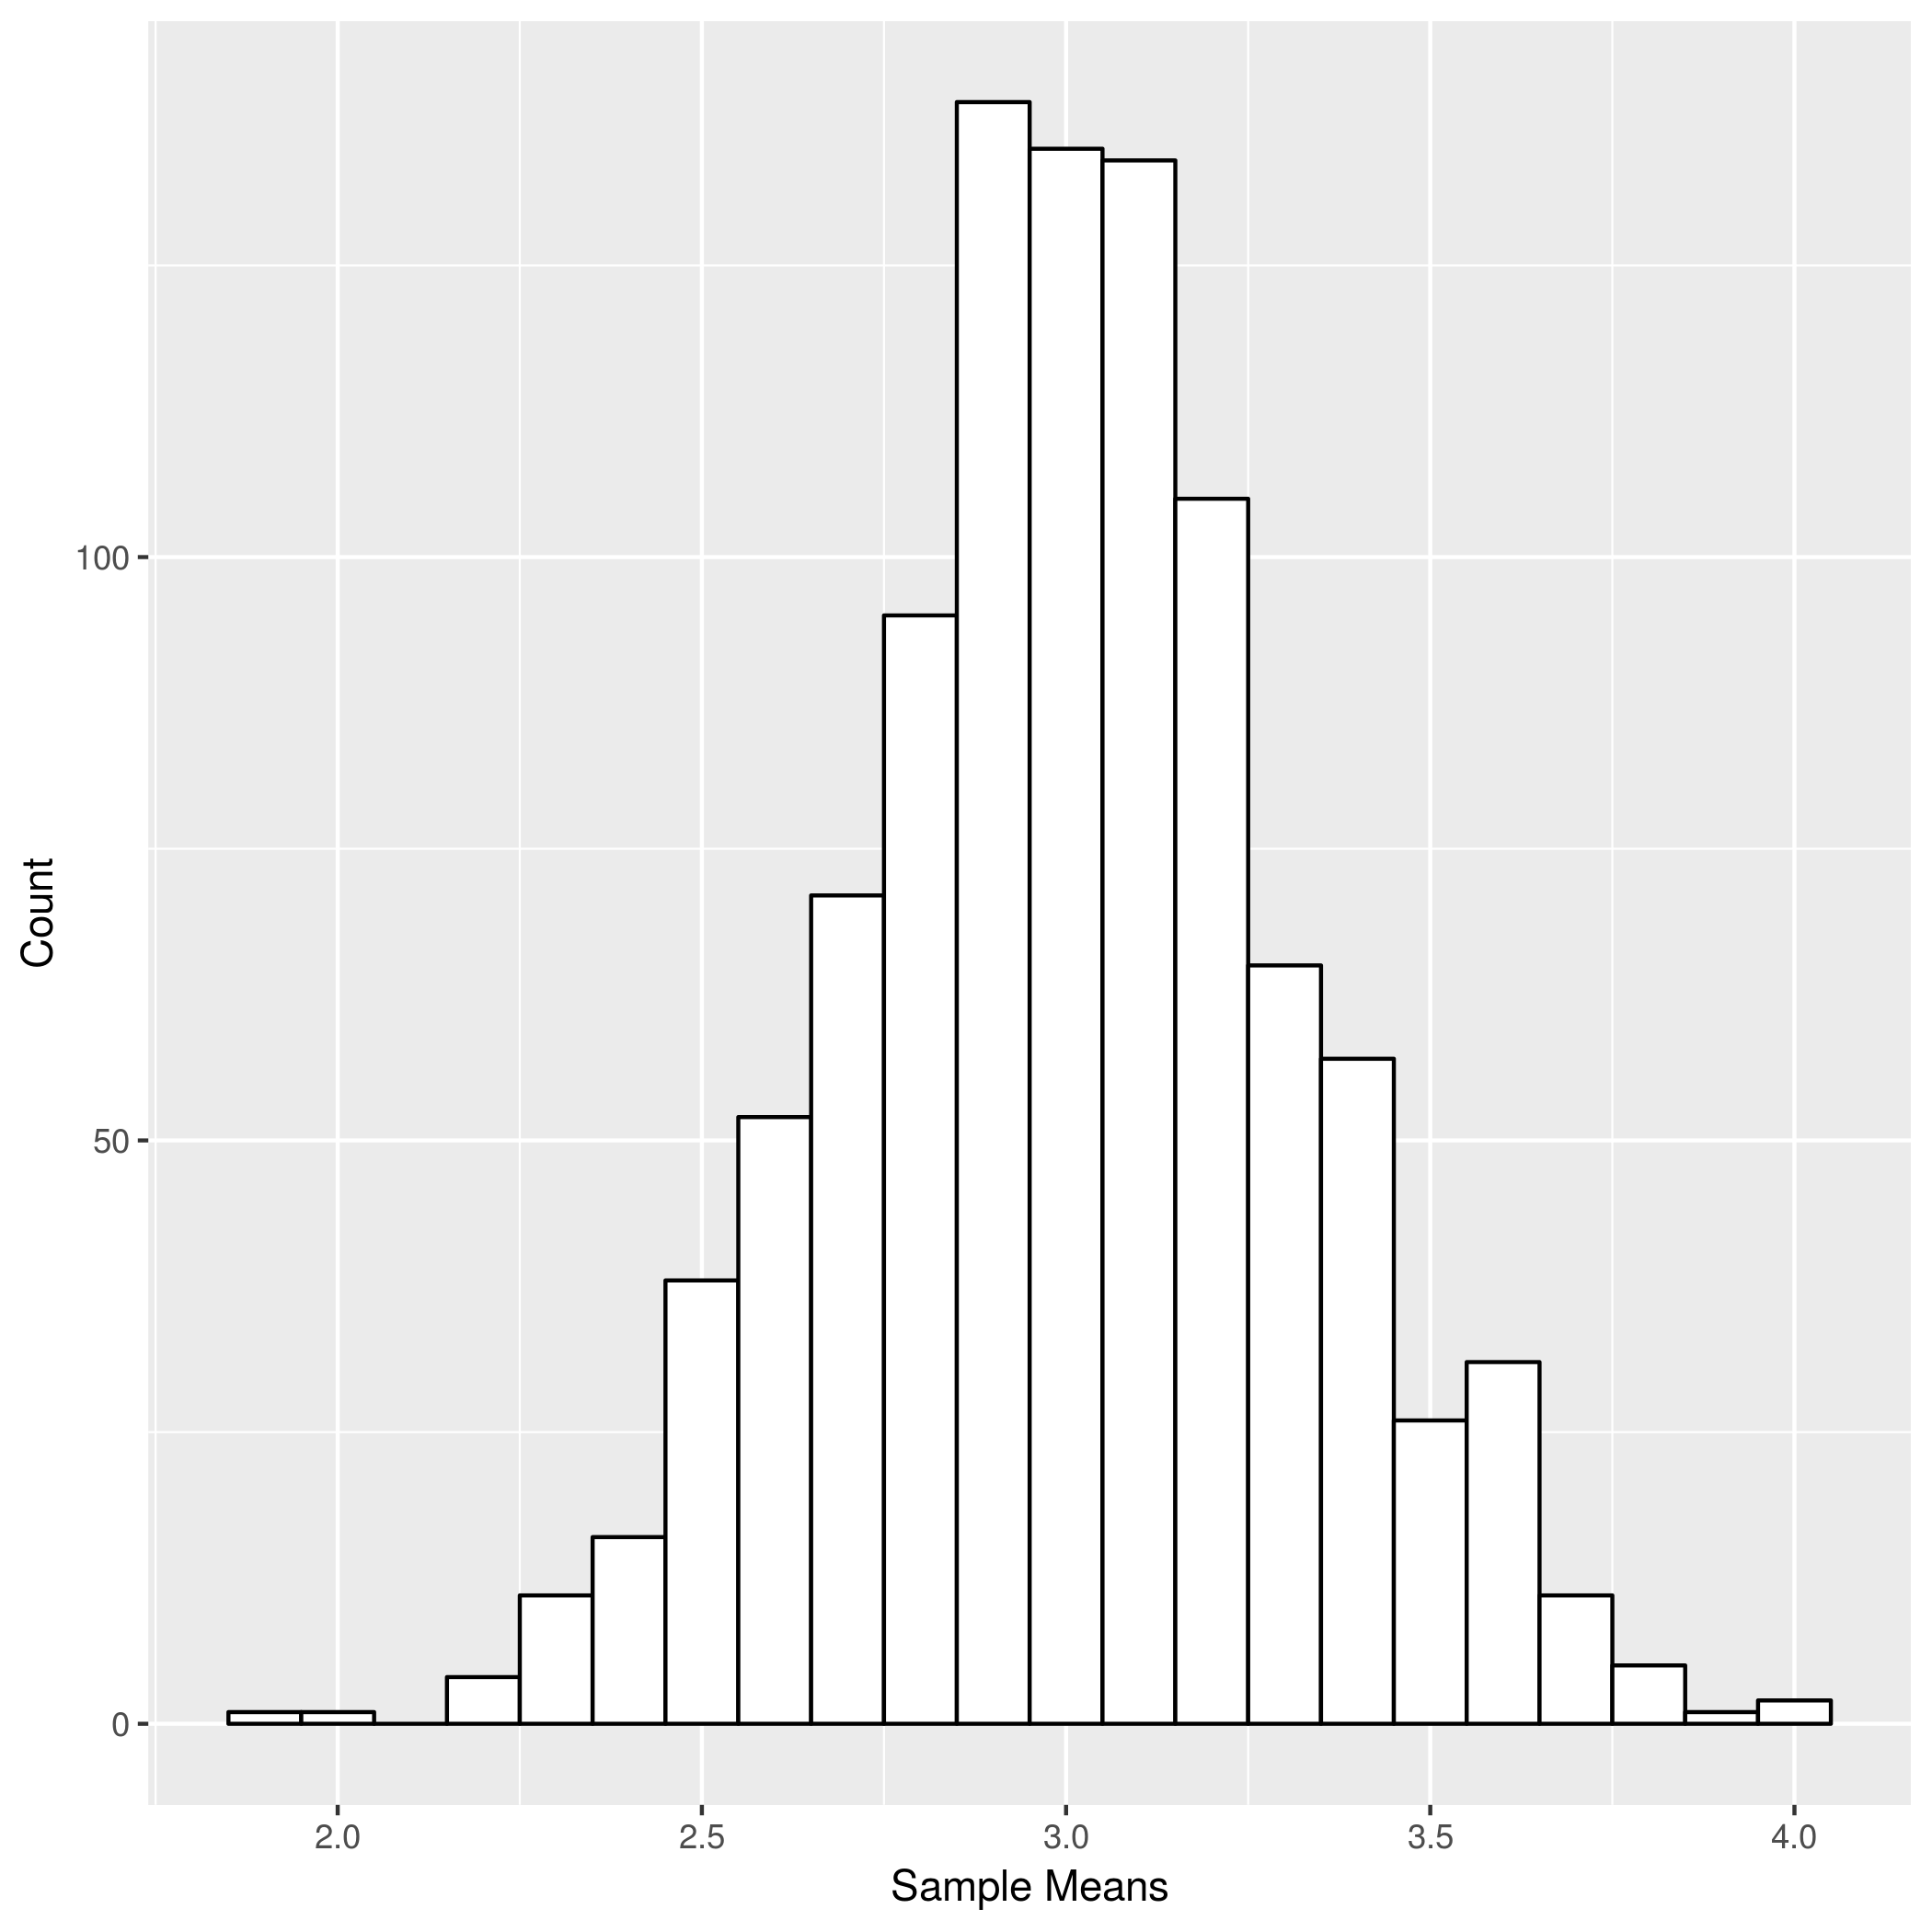
\includegraphics[width=0.5\textwidth]{figures/hist1.png}
                    \caption{Histogram of the Generated Data} \label{fig:hist1}
                \end{center}
            \end{figure}


    % ------------------------------ Part 2 ------------------------------
    \section{Part 2}
        1000 random samples of size 15 were generated from a binomial distribution with n = 10 and standard deviation p = 0.15.

\begin{lstlisting}
    # initialize parameters for binomial distribution
    N <- 15
    n <- 10
    p <- 0.15

    sampMeans <- randDist(N, n, p, "binomial", "part2.tex")
    plotHist(sampMeans, "hist2.png", 0.1)
\end{lstlisting}

        \subsection{Output}

    The first sample mean and standard deviation were computed:

    \[ E(\overline{X}) = 1.000, \ \sigma_{\overline{X}} = 0.329 \]

    All the samples were then used to find the sample mean and standard
    deviation. The theoretical values were also computed based on the
    relationships:

    \[ \mu = np \]
    \[ E(\overline{X}) = np \]
    \[ \sigma = np(1-p) \]
    \[ \sigma_{\overline{X}} = \frac{np(1-p)}{\sqrt{n}} \]


    \begin{table}[h]
        \centering
        \begin{tabular*}{200pt}{@{\extracolsep{\fill}} c c c}

        & \textbf{Actual} & \textbf{Theoretical} \\
        \hline
        $\mu$ & 1.500  & 1.500 \\
        E($\overline{X}$) & 1.518 & 1.500 \\
        $\sigma$ & 1.275 & 1.275 \\
        $\sigma$\textsubscript{$\overline{X}$} & 0.292 & 0.329 \\

        \end{tabular*}
    \end{table}


        \subsection{Distribution}
            Distribution of the data was plotted with a histogram using ggplot2 in Figure \ref{fig:hist2}.
\begin{lstlisting}
    # plot a histogram of the data
    ggplot() + aes(sampMeans) + 
        geom_histogram(binwidth=0.1, color="black", fill="white") +
        labs(y="Count", x="Sample Means")
\end{lstlisting}

            \begin{figure}[h!]
                \begin{center}
                    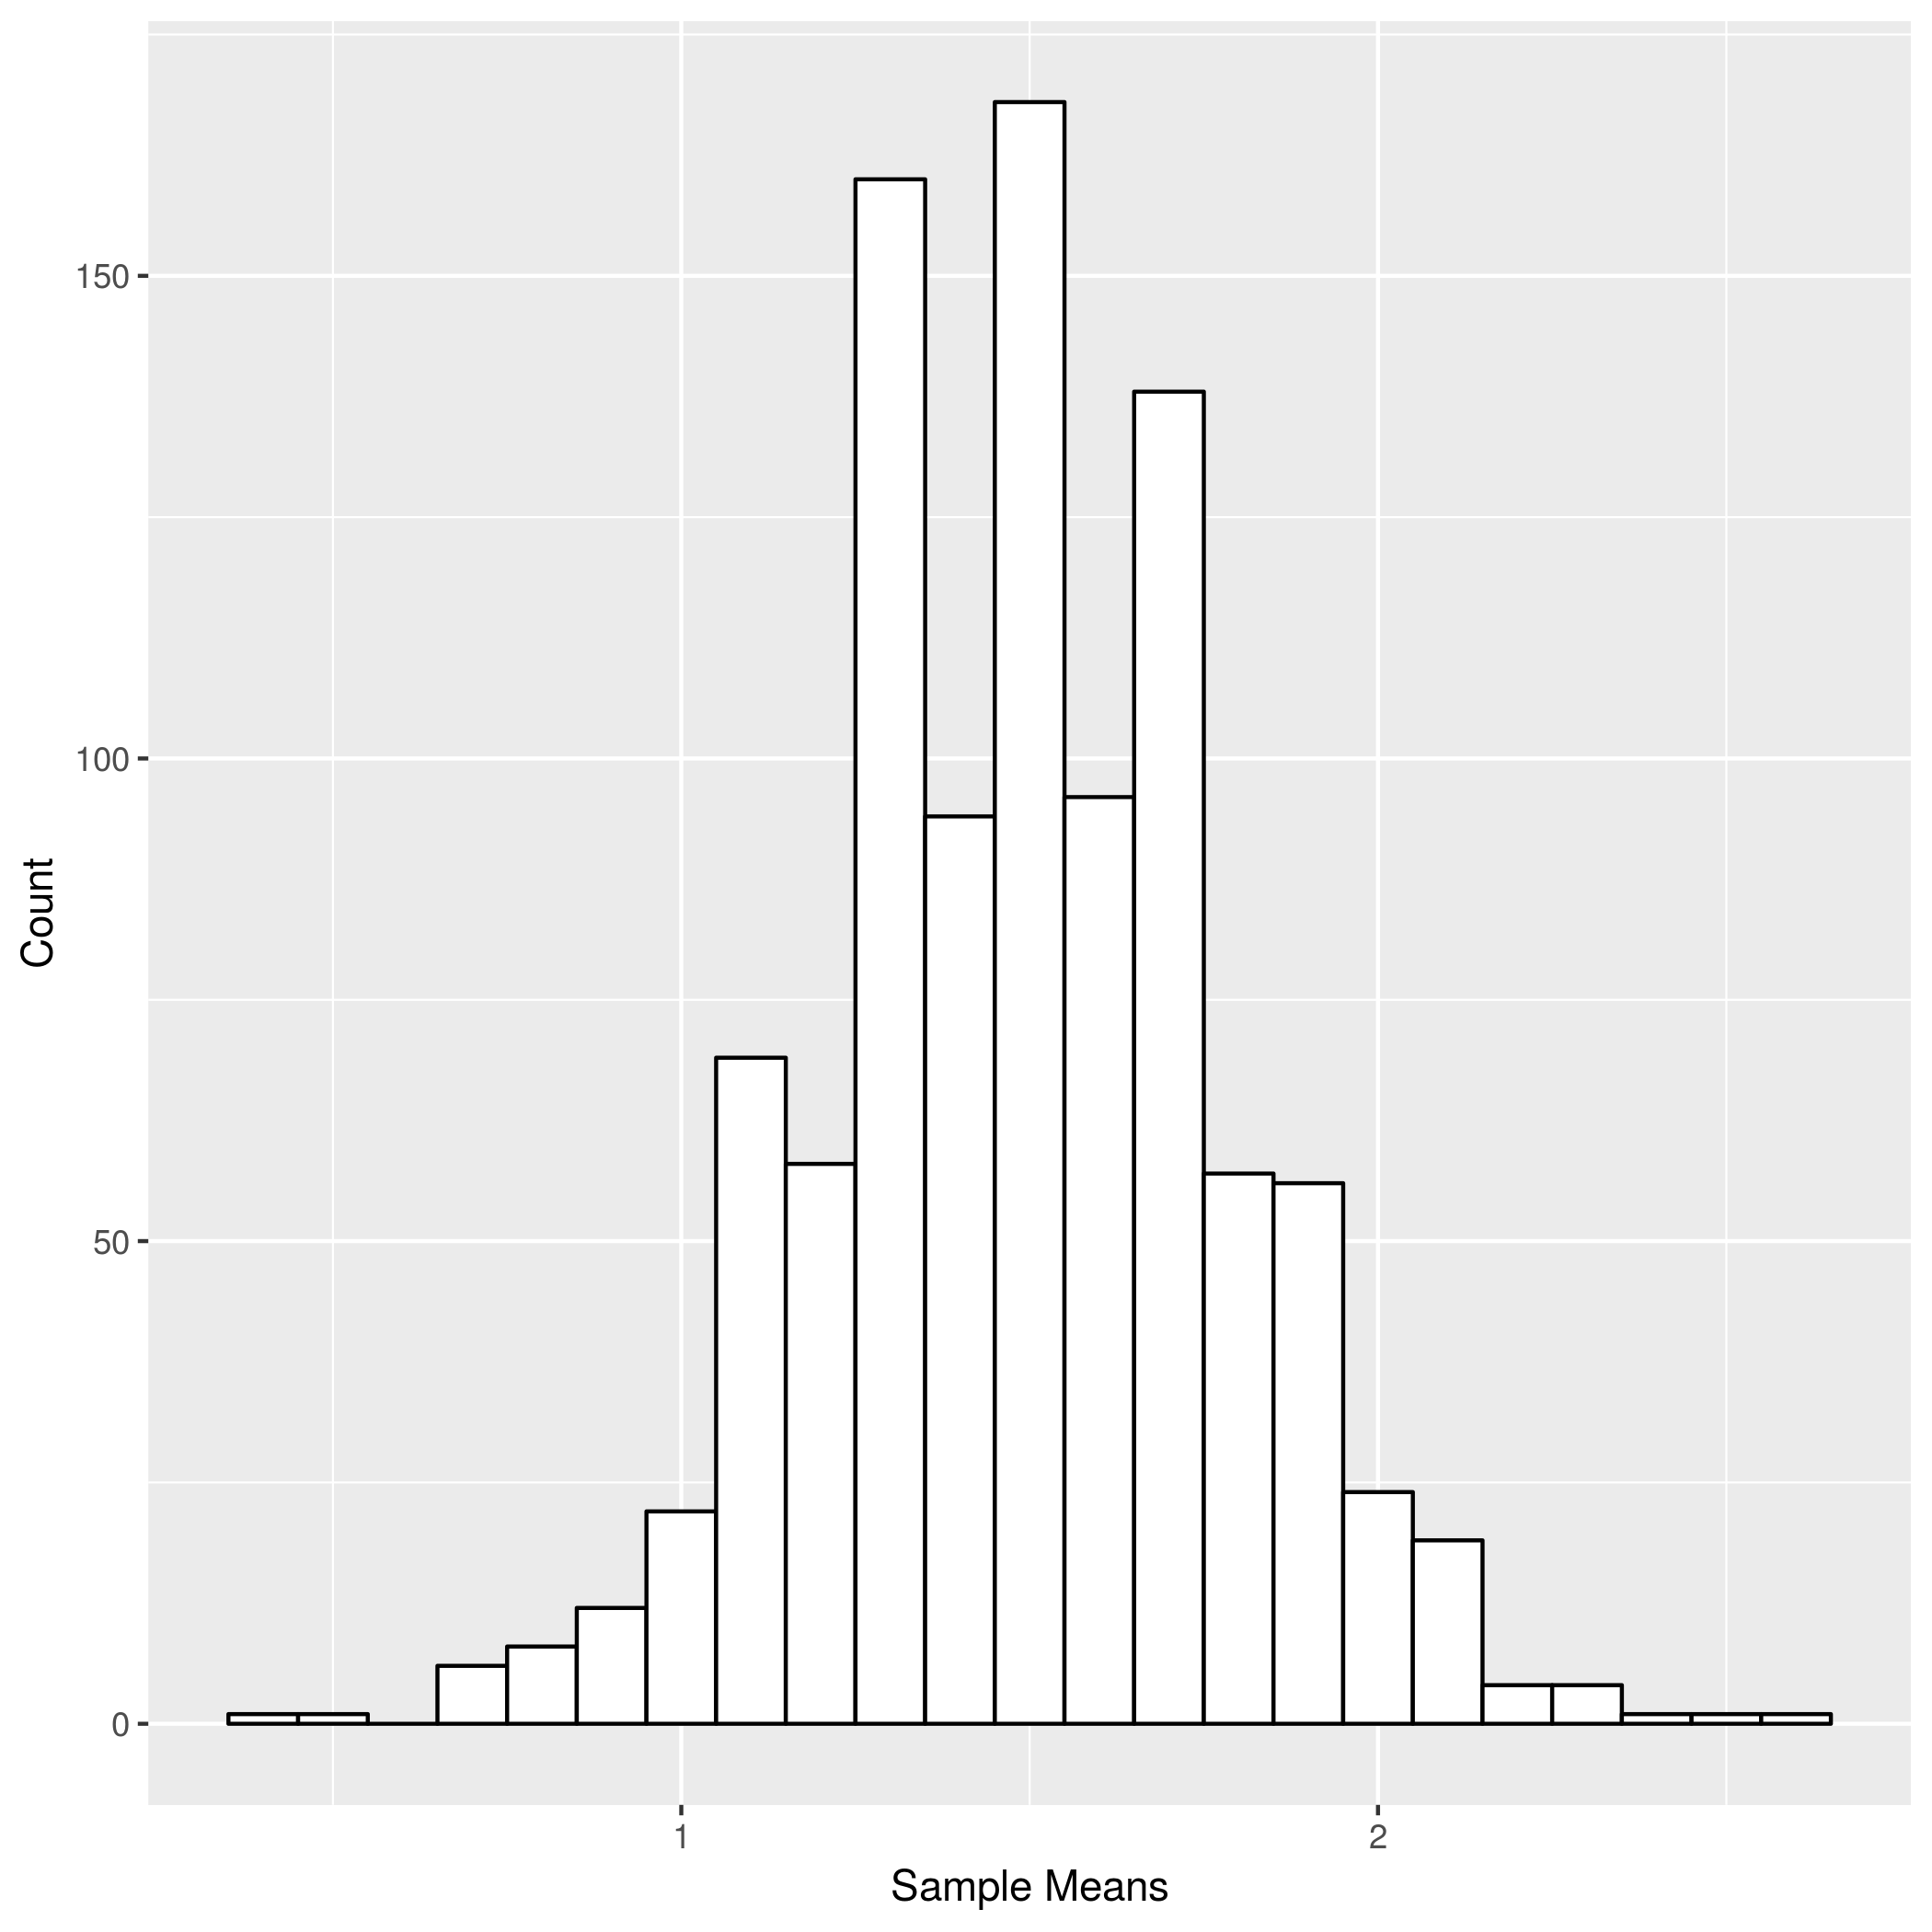
\includegraphics[width=0.5\textwidth]{figures/hist2.png}
                    \caption{Histogram of the Generated Data} \label{fig:hist2}
                \end{center}
            \end{figure}


    % ------------------------------ Part 3 ------------------------------
    \section{Part 3}
        1000 random samples of size 120 were generated from a binomial distribution with n = 10 and standard deviation p = 0.15.

\begin{lstlisting}
    # initialize parameters for binomial distribution
    N <- 120
    n <- 10
    p <- 0.15

    sampMeans <- randDist(N, n, p, "binomial", "part3.tex")
    plotHist(sampMeans, "hist3.png", 0.025)
\end{lstlisting}

        \subsection{Output}

    The first sample mean and standard deviation were computed:

    \[ E(\overline{X}) = 1.492, \ \sigma_{\overline{X}} = 0.116 \]

    All the samples were then used to find the sample mean and standard
    deviation. The theoretical values were also computed based on the
    relationships:

    \[ \mu = np \]
    \[ E(\overline{X}) = np \]
    \[ \sigma = np(1-p) \]
    \[ \sigma_{\overline{X}} = \frac{np(1-p)}{\sqrt{n}} \]


    \begin{table}[h]
        \centering
        \begin{tabular*}{200pt}{@{\extracolsep{\fill}} c c c}

        & \textbf{Actual} & \textbf{Theoretical} \\
        \hline
        $\mu$ & 1.500  & 1.500 \\
        E($\overline{X}$) & 1.502 & 1.500 \\
        $\sigma$ & 1.275 & 1.275 \\
        $\sigma$\textsubscript{$\overline{X}$} & 0.101 & 0.116 \\

        \end{tabular*}
    \end{table}


        \subsection{Distribution}
            Distribution of the data was plotted with a histogram using ggplot2 in Figure \ref{fig:hist3}.
\begin{lstlisting}
    # plot a histogram of the data
    ggplot() + aes(sampMeans) + 
        geom_histogram(binwidth=0.025, color="black", fill="white") +
        labs(y="Count", x="Sample Means")
\end{lstlisting}

            \begin{figure}[h!]
                \begin{center}
                    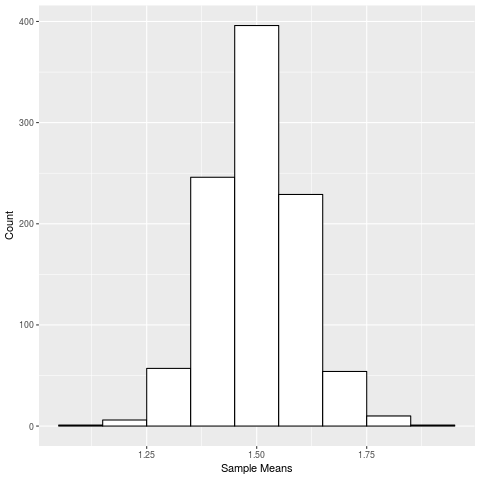
\includegraphics[width=0.5\textwidth]{figures/hist3.png}
                    \caption{Histogram of the Generated Data} \label{fig:hist3}
                \end{center}
            \end{figure}


    \section{Conclusion}
    The sample means for the normal and binomial distributions all generated normal distributions. The Part 1 distribution (Figure \ref{fig:hist1}) demonstrates a normal sample mean distribution. The theoretical sample mean and standard deviation appear very close to the computed values.\\


    For the binomial distributions, it can be observed that the distribution with the larger sample size of 150 per random sample yielded sample mean and standard deviation values much closer to their theoretical values. The larger sample size also generated a normal distribution of sample means for the binomial distribution.\\



    The normal distributions generated from the various distributions essentially demonstrated the central limit theorem, which implies a given distribution with a mean $\mu$ and standard deviation $\sigma$, the sampling distribution of the mean approaches a normal distribution with a mean ($E(\overline{X})$) and a standard deviation $\frac{\sigma}{\sqrt{N}}$ as N, the sample size, increases. \cite{wolfram}

    \begin{thebibliography}{9}

        \bibitem{wolfram}
        Central Limit Theorem
        \\\texttt{http://mathworld.wolfram.com/CentralLimitTheorem.html}

    \end{thebibliography}

    \clearpage
    \newpage
    \VerbatimInput{main.R}

\end{document}
